%!TEX root = ../data_poisoning.tex\phantomsection
\section*{Обзор современных методов атак и защиты}
\addcontentsline{toc}{section}{Обзор современных методов атак и защиты}
\subsection*{Атаки отравлением данных}
Изменить набор обучающий данных $D$ таким образом, чтобы целевое изображение $x_t \in D$, имеющее класс $C$ неверно классифицировалось в целевой класс $C'$.
При этом нужно оказать как можно меньшее влияние на классификацию остальных изображений.

В классических методах атак отравлением данных считается, что атакующий контролирует обучающий данных $D$ и может произвольно менять в нём данные в пределах $J$ примеров.

Рассмотрим наиболее распространённые методы классических атак.

\textbf{Простая замена метки класса у целевого изображения}
Очень малоэффективная атака при больших объёмах доступных для обучения данных. Зачастую модели обладают хорошей обобщающей способностью и с большой вероятностью не выучат один неверно размеченный пример.

\textbf{Feature Collision}~\cite{schwarzschild_just_2021}
Вместе с простой заменой метки класса у целевого изображения, мы пытаемся осуществить минимальное изменение изображений из целевого класса $C'$ так чтобы признаки отравленных данных были максимально близки к признакам целевого изображения.

$$x^{j}_{p} = \argmin_x ||f(x)-f(x_t)||_{2}^{2}$$

$$\text{при условии, что~} ||x_{p}^{j} - x_{b}^{j}||_{\infty} \leq \epsilon$$


\textbf{Convex Polytope}~\cite{schwarzschild_just_2021}
Вместе с простой заменой метки класса у целевого изображения, мы пытаемся сделать так, чтобы признаки целевого изображения представлялись линейной комбинацией отравленных данных из класса $C'$

$$X_p = \argmin_{c_j, x^j} ||f(x_t) - \sum_{j=1}^{J} c_j f(x^j){||}_{2}^{2}$$
$$\text{при условии~} \sum_{j=1}^{J} c_j = 1$$
$$\text{и~} c_j \geq 0~\forall j$$
$$\text{и~} ||x_{p}^{j} - x_{b}^{j}||_{\infty} \leq \epsilon$$


\textbf{Witches' Brew via gradient matching}~\cite{geiping_witches_2021}
При данной атаке нам дополнительно известна архитектура обучаемой модели $F(x, \theta)$ и её функция потерь $L(y_{pred}, y_{true})$.
Вместе с простой заменой метки класса у целевого изображения, мы отравляем данные из класса $C'$ так чтобы вектора градиентов функции потерь для них были сонаправлены с вектором градиента функции потерь для целевого изображения.

$$\nabla_{\theta} L(F(x_t, \theta), C') \uparrow\uparrow \nabla_{\theta} L(F(x_{p}^{j}, \theta), C')$$
$$\text{где~} x_{p}^{j} = x_{b}^{j} + \delta_j \text{~и~} ||\delta_j||_{\infty} \leq \epsilon$$

\vspace{25pt}

Помимо классической модели угроз, также рассматривают модель угроз, в которой атакующий ограничен в возможножсти чтения обучающих данных. \\
В атаках без возможности чтения обучающих данных (также называются атаки методом чёрного ящика) ожидается, что атакующий не имеет доступа к обучающему набору данных, однако знает из какого они распределения и имеет возможность выбирать данные из этого распределения неограниченно, либо по определённым правилам. Также атакующий знает структуру обучаемой модели, её функцию потерь и имеет возможность внедрять отравленные данные в обучающий набор данных для конечной модели.

Рассмотрим наиболее распространённые методы таких атак.

\textbf{Subpopulation Attack}~\cite{jagielski_subpopulation_2021}
Идея заключается в следующем: мы выбираем большое количество данных из известного нам распределения исходных данных. Затем проводим кластеризацию.

Кластеризацию можно производить:
\begin{itemize}
    \item Вручную по высокоуровнему признаку: например наличия на картинке какого-либо элемента;
    \item Автоматически путём предварительной фильтрации и кластеризации либо оригинальных изображений, либо извлечённых признаков.
\end{itemize}

Кластеризацию следует производить таким образом, чтобы кластер с целевым изображением имел размер не более чем $J$. Затем мы меняем метку на $C'$ для всего кластера и отправляем получившиеся данные на обучение модели.

% TODO: описать оптимизацию атаки

\textbf{Online Learning Attack}~\cite{zhang_online_2020}
В атаке предполагается что модель обучается в режиме реального времени и атакующему известно текущие веса модели. В каждый момент времени атакующий получает обучающий пример и у него есть два варианта действия:
\begin{itemize}
    \item Передать пример модели;
    \item Модифицировать пример и передать модели.
\end{itemize}

При этом атакующий не может менять принятого ранее решения.

Задачу можно переформулировать в виде марковского процесса принятия решений, введя функцию штрафов $g(s_T, x_T)$, где $s_T$ – текущее состояние, описываемое положением в марковском процессе и весами модели, $x_T$ – пример, доступный в момент времени $T$.

\noindentТогда ожидаемый штраф для атакующего будет составлять:
$$V_{\mathcal{M}}^{\phi}(\mathbf{s}):=\left.\mathbb{E}_{\mathcal{M}} \sum_{T=0}^{\infty} \gamma^{T} g\left(\mathbf{s}_{T}, \phi\left(\mathbf{s}_{T}\right)\right)\right|_{\mathbf{s_0}=\mathbf{s}}$$
Где $\gamma$ – дисконтирующий множитель, введённый для решения проблемы с неограниченностью процесса по времени.


\noindentА оптимальная политика действий:
$$
\phi* = \argmin_{\phi} \mathbb{E}_{\mathbf{S} \sim \mu_{0}} V_{\mathcal{M}}^{\phi}(\mathbf{s})
$$

\subsection*{Атаки внедрением триггера (Backdoor)}
Атаки внедрением триггера ставят своей целью изменить набор обучающий данных $D$ таким образом, чтобы любое изображение, при наложении на него специального триггера классифицировалось в целевой класс $C'$.
При этом, также как и в случае обычных атак отравлением, нужно оказать как можно меньшее влияние на классификацию остальных изображений.

Примером триггера может быть помещение небольшого квадрата из чёрных или цветных пикселей в угол изображения.

\textbf{Простая замена метки класса у отравленных изображений}
Также как и в случае обычных атак отравлением данных этот способ работает малоэффективно по тем же причинам.

\textbf{Clean-label backdoor}~\cite{zhao_clean-label_2020}
Замена метки плоха ещё и тем, что посмотрев глазами на изображение можно легко убедиться, что на нём изображено не совпадает со значением метки класса.

Атака Clean-label backdoor заключается в том, чтобы уменьшить значимость всех иных признаков и заставить модель обращать максимальное внимание на триггер. Триггер при этом накладывается только на изображения класса $C'$, и таким образом метки классов остаются без изменения.

Для достижения поставленной цели могут быть использованы генеративные состязательные нейронные сети.
Пусть $G(z)$ – генератор, где $z$ – латентное представление изображения размерности $d$.

\noindentТогда найти латентное представление изображения $x$ можно по формуле:
$$E_{G}(x)=\arg \min _{z \in \mathbb{R}^{d}}\|x-G(z)\|_{2}$$

\noindentМы также можем сделать сдвиг в пространстве латентных представлений между двумя изображениям:
$$I_{G}\left(x_{1}, x_{2}, \tau\right)=G\left(\tau z_{1}+(1-\tau) z_{2}\right)$$

Где $\tau$ должно быть достаточно большим, чтобы снизить значимость признаков изображения, но достаточно маленьким, чтобы не быть заметным человеческому взгляду в отсутствии оригинала для сравнения.

% TODO: описать Adversarial examples bounded in `p-norm

\textbf{Hidden-trigger backdoor}~\cite{HiddenTrigger}
В атаке решается следующая оптимизационная задача:
$$
\begin{array}{r}
\arg \min \|f(z)-f(\tilde{s})\|_{2}^{2} \\
\text{при условии~} \quad\|z-t\| \|_{\infty}<\epsilon
\end{array}
$$
Где $z$ – отравленное изображение, которое будет помещено в обучающий набор данных; $\tilde{s}$ – изображение из класса $C$ с наложенным на него триггером; $t$ – изображение из класса $C'$.

% \textbf{Deep Feature Space Trojan}
% Идея заключается в том чтобы сделать триггер более незаметным: для стороннего наблюдателя картинки с триггером и без него должны быть идентичны.
% Также триггер не должны обнаруживать системы, которые полагаются на
% то, что отравленные модели переобучаются на простые триггеры.
% TODO: разобраться можно ли применить без контроля обучения модели

\subsection*{Методы защиты}
\textbf{Поиск отравленных примеров при помощи кластеризации}~\cite{chen_detecting_2018}
Идея метода детектирования: провести тренировочный набор данных через
обученную нейронную сеть и набор векторов активаций последнего скрытого
слоя. Этот набор разбивается по классам и в каждом классе отдельно хорошо
разделяется на кластеры соответствующие отравленным и чистым данным.
При этом перед кластеризацией используется PCA с проекцией на 3 первых
компоненты.

Самым эффективным методом кластеризации выбран k-means с $k=2$ Далее для проверки, что данные отравлены мы можем исключить какой-нибудь
кластер из обучающего множества и затем провести его через новый классификатор. Если большая доля примеров попадает в один конкретный неверный
класс, то это подозрительно и требует проверки.
Также когда отравленных данных $p\%$, то размер кластера, соответствующего им будет составлять примерно $p\%$. Если же отравленных данных нет,
то размеры кластеров будут примерно равны. С той же целью можно использовать silhouette score.
Также мы можем составить усреднённый пример из кластера и проверив его вручную сделать вывод о наличии отравления: например триггеры атак внедрения backdoor могут сильно выделяться.
Для исправления модели предлагается изменить метки отравленным
классам и дообучить модель на исправленных данных.

\textbf{Поиск отравленных примеров при помощи Auto Encoder моделей}~\cite{razmi_classification_2021}
Модель Auto Encoder можно использовать для детектирования сильных аномалий, потому что он не может их точно восстановить. Но для этого Auto Encoder должен Быть обучен на доверенном наборе данных.

Однако в чистом виде этот метод обладает несколькими недостатками:
\begin{itemize}
    \item Отравление часто происходит малыми изменениями, что может быть незаметным для Auto Encoder модели;
    \item Такой подход не анализирует метки классов, а они могут быть изменены;
    \item Требование доверенного набора данных накладывает существенные ограничения на применимость этого метода.
\end{itemize}
Для решения этих проблем был разработан метод под названием "Classification Auto-Encoder based detector $+$ (CAE+)".

\begin{figure}[h]
    \center{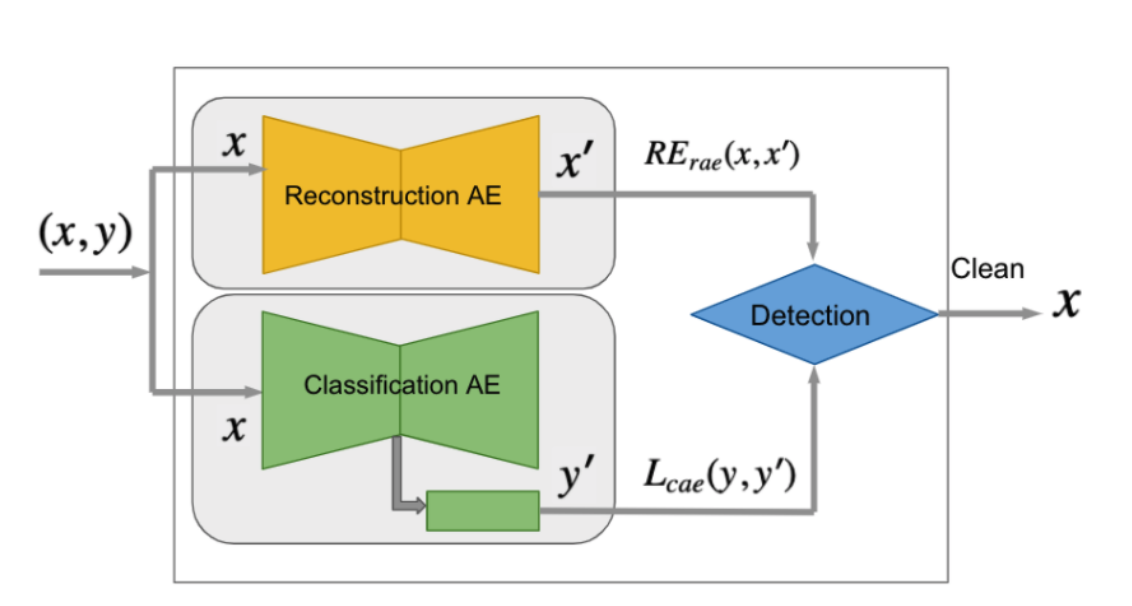
\includegraphics[scale=0.5]{cae_plus.png}}
    \caption{Схема устройства CAE+}
    \label{cae_plus_image}
\end{figure}

На рисунке \ref{cae_plus_image} изображена схема модели CAE+. Classification Auto Encoder получает внутреннее представление изображение (embedding) и предсказывает по нему метку класса изображению. Reconstruction Auto Encoder получает отдельное внутреннее представление изображения и пытается восстановить из него исходное изображение. В случае, если взвешенная ошибка на каком-либо изображении превышает заданный порог, мы подозреваем, что это изобржание может быть отравлено.

Этот метод может обучаться даже на недоверенном наборе данных. В этом случае для предотвращения переобучения на отравленные данные процесс обучения прерывается раньше чем обычно.


\textbf{Сертификация робастности модели}~\cite{jia_intrinsic_2020}

Для некоторых моделей возможно доказать их устойчивость к отравлениям. Например для Bagging классификатора.
Обучающие подмножества для каждого базового классификатора выбираются случайно. Процесс обучения тоже носит стохастический характер.

Теоретическое определение вероятности того, что предсказанная метка при отравлении не изменится, получается при помощи леммы Неймана-Пирсона.
Определяется нижняя граница вероятности наиболее вероятного
предсказания и верхняя граница вероятности второго по вероятности предсказания для того чтобы при отравлении $r$ примеров не произошло изменений в предсказании.

$r$ получается как решение оптимизационной задачи.

%TODO описать задачу


\textbf{Метод очистки отравленной модели GangSweep}~\cite{zhu_gangsweep_2020}
Ключевым понятием этого метода является "изменяющая маска" – минимальное попиксельное изменение изображения, при котором модель начинает классифицировать изображение из класса $C$ как изображение из класса $C'$.

По результатам экспериментов, внедрение backdoor слабо изменяет дисперсию в пространстве признаков, но сильно изменяет расстояние.

Состязательные нейросети при генерации изменяющей маски очень хорошо перебирают
пространство вокруг объекта. В методе используется состязательная сеть
для генерации изменяющей маски от каждого класса к каждому.
Если в модель внедрён Backdoor, то для различных изображений изменяющие маски к целевому классу будут очень близки.

Отфильтровать изменяющие маски для последующего анализа можно посредством алгоритма z-score, для того чтобы выделить те, которые слабо изменяют дисперсию, но сильно изменяют расстояние в пространстве признаков.

% TODO: добавить изображения
